\documentclass[10pt]{beamer}

\usepackage[T2A]{fontenc}
\usepackage[utf8]{inputenc}
\usepackage[russian,english]{babel}

\usefonttheme[onlymath]{serif}

\usetheme[progressbar=frametitle]{metropolis}
\usepackage{appendixnumberbeamer}

\usepackage{booktabs}
\usepackage[scale=2]{ccicons}

\usepackage{pgfplots}
\usepgfplotslibrary{dateplot}

\usepackage{xspace}
\newcommand{\themename}{\textbf{\textsc{metropolis}}\xspace}
\newcommand{\TODO}[1]{\textbf{\textcolor{red}{TODO: #1}}}

\date{}
\author{Екатерина Тузова}


\title{Лекция 4}
\subtitle{Деревья принятия решений}

\begin{document}

\maketitle

\section{Разбор летучки}

\begin{frame}{}
	\centering
	\begin{figure}
		\begin{minipage}{.5\textwidth}
		  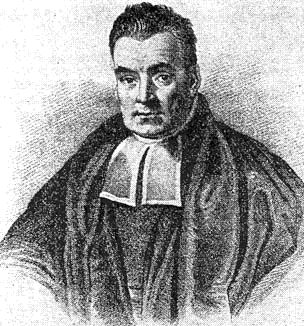
\includegraphics[width=0.9 \linewidth, height=150pt, keepaspectratio]{images/bayes}
		\end{minipage}%
		\begin{minipage}{.5\textwidth}				
			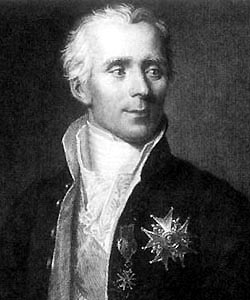
\includegraphics[width=0.9 \linewidth, height=150pt, keepaspectratio]{images/laplace}
		\end{minipage}
	\end{figure}
\end{frame}

\section{Мотивирующий пример}

{\foot{\href{http://qwone.com/~jason/20Newsgroups}{http://qwone.com/~jason/20Newsgroups}}
\begin{frame} {Классификация сообщений}
  Датасет \alert{20 newsgroups} содержит почти 20000 сообщений из списков рассылки Usenet.\\
  \pause
  \bigbreak
  Примеры сообщений из списка рассылки sci.crypt:\\
  \begin{quotation}
    When you find out a floppy password protect program, could you e-mail me.\\
    Thanks\\
    \bigbreak
    Not to mention Computer Associates. I'll have to be careful to stop telling people I'm a Clipper programmer, they might lynch me... :-)
  \end{quotation}
  \pause
  \alert{Задача}: Построить классификатор, предсказывающий по тексту сообщения список рассылки, в который оно было отправлено.
\end{frame}
}

\begin{frame} {Вероятностная постановка задачи}
  $X$ -- множество объектов\\
  $Y$ -- множество меток классов\\
  $X \times Y$ -- вероятностное пространство с плотностью \\
  $$p(x,y) = P_yp(x|y)$$\\
  \bigbreak
  $P_y$ -- априорная вероятность класса $y$\\
  $p(x|y)$ -- функция правдоподобия класса $y$\\
  \bigbreak
  \pause
  \alert{Задача}: Построить алгоритм $a: X \rightarrow Y$, минимизирующий \textbf{вероятность} ошибки.
\end{frame}

\begin{frame}{Известное и неизвестное}
  Как правило, априорные вероятности $P_y$ и функции правдоподобия классов $p(x|y)$ неизвестны.\\
  \pause
  \bigbreak
  2 подзадачи:
  \begin{enumerate}
    \item По выборке $X^l$ из неизвестного распределения с плотностью $p(x, y)$ построить оценки вероятностей $\hat{P}_y$ и функций правдоподобия $\hat{p}(x|y)$ для каждого класса
    \item По известным $P_y$ и $p(x|y)$ построить функцию $a(x)$, минимизирующую вероятность ошибочной классификации
  \end{enumerate}
\end{frame}

\begin{frame}{Вопрос}
  \centering
  Предположим, что нам известно заранее распределение с плотностью $p(x, y)$. Как оценить вероятность ошибочной классификации для произвольного алгоритма $a: X \rightarrow Y$?
\end{frame}

\begin{frame}{Функционал среднего риска}
  $\lambda_{ys}$ -- штраф за назначение класса $s$ объекту $y$\\
  \pause
  \bigbreak
  \alert{Полезные} нам значения $\lambda_{ys}$ такие, что $\lambda_{yy} = 0$ и $\lambda_{ys} > 0$ для всех $y \neq s$.
  \pause
  \bigbreak
  Функционал среднего риска алгоритма $a$:\\
  $$R(a) = \sum\limits_{s \in Y} \sum\limits_{y \in Y} \lambda_{ys} P_y p(A_s|y) \qquad p(A_s|y) = \int\limits_{A_s} p(x|y) dx$$\\
  $A_s = \left\{ x \in X | a(x) = s \right\}$ -- множество объектов класса $y$, которым алгоритм ошибочно назначил класс $s$
\end{frame}

\begin{frame}{Функционал среднего риска}
  Функционал среднего риска алгоритма $a$:\\
  $$R(a) = \sum\limits_{s \in Y} \sum\limits_{y \in Y} \lambda_{ys} P_y p(A_s|y) \qquad p(A_s|y) = \int\limits_{A_s} p(x|y) dx$$\\
  $A_s = \left\{ x \in X | a(x) = s \right\}$ -- множество объектов класса $y$, которым алгоритм ошибочно назначил класс $s$\\
  \bigbreak
  \pause
  $\lambda_{ys} = \left[ y \neq s \right]$, то $R(a)$ -- вероятность ошибки алгоритма $a(x)$
\end{frame}

{\foot{Optimal Bayes Classifier}
\begin{frame}{Оптимальный Байесовский классификатор}
  Минимум среднего риска $R(a)$ достигается при:\\
  $$a(x) = \arg\min\limits_{s \in Y} \sum \limits_{y \in Y} \lambda_{ys} P_y p(x|y)$$\\
  \bigbreak
  \pause
  Пусть величина штрафа зависит только от класса $y$, т.е. $\lambda_{yy} = 0$ и $\lambda_{ys} = \lambda_y$, тогда оптимальный алгоритм:\\
  $$a(x) = \arg\max\limits_{y \in Y} \lambda_y P_y p(x|y)$$
\end{frame}
}

\end{document}